\documentclass[conference]{acmsiggraph}

\TOGonlineid{45678}
\TOGvolume{0}
\TOGnumber{0}
\TOGarticleDOI{1111111.2222222}
\TOGprojectURL{}
\TOGvideoURL{}
\TOGdataURL{}
\TOGcodeURL{}

\title{Ray Tracing Implicit Surfaces}

\author{David Rusk\thanks{e-mail:drusk@uvic.ca}\\University of Victoria}
\pdfauthor{David Rusk}

\keywords{ray tracing, implicit surfaces}

\begin{document}

\maketitle

\begin{abstract}

A ray tracer for rendering implicit surfaces was developed from scratch.
It guarantees ray intersections will be found by requiring upper 
bounds L and G, which limit the rates of change of the implicit function 
and its derivative, respectively.

\end{abstract}

\keywordlist

%% Use this only if you're preparing a technical paper to be published in the 
%% ACM 'Transactions on Graphics' journal.

\TOGlinkslist

%% Required for all content. 

\copyrightspace

\section{Introduction}

Implicit surfaces are a method for modelling objects using an equation
where the function is set to equal 0.  There are two ways in which to
render these surfaces: polygonization and ray tracing.  Polygonization
involves breaking down the surface into polygons and rendering them, 
while ray tracing calculates the values of the pixels in the image
one-by-one.  This project investigates using the second technique, 
ray tracing, for rendering implicit surfaces.

The challenge when ray tracing implicit surfaces is reliably finding
ray intersections with the surface.  The techniques of Kalra and
Barr \cite{KalraBarr1989} were used to guarantee the success of this
process, as long as upper bounds on the net rate of change of the 
implicit function and its derivative are known.  

Kalra and Barr describe two steps to their algorithm.  The first is a
space pruning algorithm which narrows down the search space for 
ray intersections.  The second is the ray intersection algorithm 
itself.  These algorithms will be explained in detail in section 
\ref{sec:Algorithms}.

\section{Background}

Real time ray tracing of implicit surfaces has also become an active
area of research recently.  Singh and Narayanan \cite{RealTimeGPU} 
have developed a GPU-based real time implicit surface ray tracer.
Knoll et al. \cite{RealTimeIntervals} have developed 
a real time implicit surface ray tracer using SIMD optimized interval 
arithmetic and coherent ray traversal.  They claim it is able to
render any programmable implicit function based only on its definition
in real time without special hardware.

\section{Methodology}

This section will give some background information about ray tracing,
implicit surfaces, and LG surfaces, which will be useful for 
understanding the algorithms used in this project.

\subsection{Ray Tracing}

Rendering three-dimensional objects is a fundamental task in computer 
graphics.  The goal is to take a scene of three-dimensional objects 
and produce a two-dimensional image showing the objects as viewed
from a specific location.  In particular, the input is a set of 
objects and the output is an array of pixels.

There are two ways to consider how each object contributes to each 
pixel: object-ordered rendering and image-ordered rendering.  In
object-ordered rendering iteration is over the objects, and for
each object all the influenced pixels are found and updated.  In
image-ordered rendering iteration is over the pixels, and for each
pixel the objects that affect it are found and used to calculate
that pixel's value.

Ray tracing is an image-ordered rendering technique.  For each pixel
it follows these steps:
\begin{enumerate}
	\item Compute the ray from the camera to the current pixel.
	\item Find the first object the ray intersects.
	\item Use the intersection point, the object's surface normal at that
	point, and any lighting, to calculate the pixel value.
\end{enumerate}

For more reading about ray tracing, see Shirley et al. \cite{Shirley}.

\subsection{Implicit Surfaces}

Implicit surfaces are a method for modelling objects using an equation
where the function is set to equal 0.  For example, here is the 
equation describing a sphere:

\begin{equation}
f(x, y, z) = x^2 + y^2 + z^2 - r^2 = 0
\end{equation}

In this case the value of the function will be negative inside the 
sphere, positive outside, and 0 on the boundary.

In order to render the implicit surface, points in space are sampled
to see whether they are inside, outside, or on the border.  This process
is expensive to evaluate, but it has some advantages.  For more information,
see Shirley et al. \cite{Shirley}.

\subsection{LG Surfaces}

Kalra and Barr \cite{KalraBarr1989} point out that it is not possible to
guarantee correct intersection of a ray with an arbitrary implicit surface
just using evaluation of the implicit function at sampled points in space.
This is because if the sampling is not fine grained enough, features that
are smaller than the distance between samples will be missed.

Therefore, extra information is needed to guarantee the intersections.
Kalra and Barr use Lipschitz constants to put bounds
on the net rate of change of the implicit function and its derivative along
the direction of the ray.

A Lipschitz constant is a constant that satisfies the following inequality:
\begin{equation}
||f(x_1) - f(x_2)|| < LipschitzConstant * ||x_1 - x_2||
\end{equation}

Let f(x) be the implicit function, and let a ray be defined by its direction 
and origin as follows:
\begin{equation}
x = \alpha * t + \beta
\end{equation}

Then the implicit function's value along the ray is:
\begin{equation}
F(t) = f(\alpha * t + \beta)
\end{equation}

The derivative of the original implicit function along the ray direction is 
then:
\begin{equation}
g(t) = dF/dt
\end{equation}

Then let L be the Lipschitz constant for f(x), and let G be the Lipschitz
constant for g(t).  Using this background information, an LG surface can
then be defined as an implicit function where L and G exist and can be
computed.  Kalra and Barr's algorithm guarantees correct ray intersections
for LG surfaces.

\section{User Interface}

The current implementation does not have an interactive graphical user 
interface because ray tracers generally are not used in real time,
though that is an active area of research (see references in the Background
section).  Instead the application is run from the command line with constant 
parameters such as image dimensions defined in a special header file.
The scene to be rendered is also currently specified directly in the 
code.  This is less than ideal because it requires recompiling the project to 
change the scene.  Some domain specific language should be developed
for specifying the scene, which the application can parse and
use to build the scene.  It should also be possible to pass arguments
on the command line to change the different parameters like
image dimensions.

\section{Data Structures}

Write data structures description here.

\section{Algorithms}
\label{sec:Algorithms}

Write algorithms description here.

\section{Implementation}

There are many open source ray tracers available on the internet.  However, 
for pedagogical reasons it was decided to implement a simple ray tracer from 
scratch.  This also made it easier to modify and adapt to support implicit
surfaces because many of the open source ray tracers are part of larger 
packages or have a lot of additional functionality.

The implementation was done in C++ and used no external libraries.  Output 
images were written to PPM \cite{PPM} files because the PPM format is 
very simple and can be implemented trivially without external libraries.

The project source code is available online at 
https://github.com/drusk/ImplicitRayTracer

\section{Results}

The system developed can currently render spheres with adjustable locations,
radii, colours, reflectivity and transparency.  The below figure shows a
simple example.  The ground is made using a sphere with a very large radius.
The light source (not in the field of view) is also a sphere.  Except for the
ground sphere, all of them are reflective.  Only the green sphere has some
transparency.

\begin{figure}[ht]
  \centering
  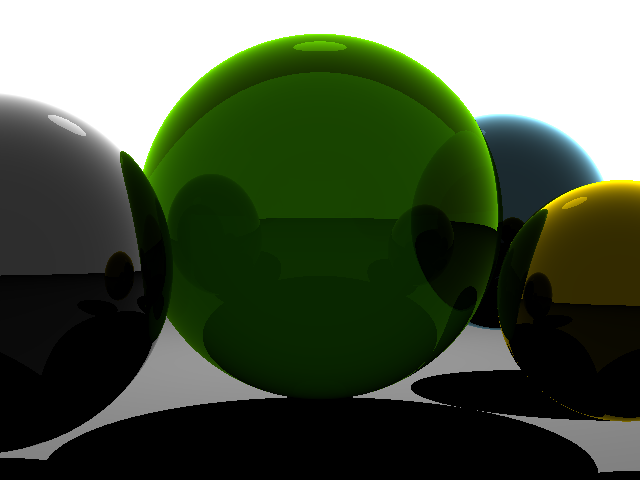
\includegraphics[width=1.5in]{figures/spheres.png}
  \caption{Example of ray traced spheres.}
\end{figure}

\section{Conclusion}

An implicit surface ray tracer was developed from scratch with no external
dependencies.  It uses the techniques of Kalra and Barr \cite{KalraBarr1989}
to find guaranteed ray intersections with the implicit surfaces.  This is done
by using two values: "L" which is an upper limit on the rate the implicit
function changes at, and "G" which is an upper limit on the rate the gradient
changes at.  This is significant because it opens up ray tracing as an 
alternative to polygonization when rendering implicit surfaces.

\section{Future Work}

A major area of future work is calculating the Lipschitz constants L and G
for other useful implicit functions.  Kalra and Barr \cite{KalraBarr1989} 
mention a forthcoming report with additional Lipschitz constants, but to
our knowledge no report was ever published.  This will allow new types of
surfaces to be rendered, and greatly increase the utility of implicit 
surfaces for modelling when using ray tracing.

Future development of the application could add support for blending surfaces
which are close to each other.  A simple two-dimensional example of this concept
is shown below.

\begin{figure}[ht]
  \centering
  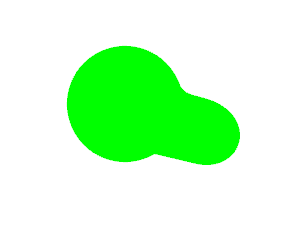
\includegraphics[width=1.5in]{figures/blend2d.png}
  \caption{Two-dimensional blend of two circles.}
\end{figure}

Adding constructive solid geometry (CSG) operations would also be useful
for modelling more advanced structures.  CSG combines primitives like 
spheres and cylinders by using the boolean set operations union,
intersection and difference.

\bibliographystyle{acmsiggraph}
\bibliography{ImplicitSurfacesRayTracer}
\end{document}

